\section{HASONLÓ FEJLESZTÉSEK VIZSGÁLATA}

A projektem két könnyen körül határolható problémát fog megoldani, így
magát az irodalom kutatásit is ily módon fogom megközelíteni. Az
elkövetkezendőkben először az útfelületi hibák detektálásával, azt
követően a detektált hibák úton belüli lokalizálásával fogok foglalkozni.

\subsection{Klasszikus képfeldolgozáson alapuló úthibadetektálás}
\label{klasszikus-kepfeldolgozason-alapulo-uthibadetektálas}

\subsubsection{Pothole detection in asphalt pavement images}
\label{pothole-detection-in-asphalt-pavement-images}

Koch Christian és Brilakis Ioannis egy 2D-s képeken alapuló eljárást
javasoltak 2011-ben, amely a kátyúk három fő vizuális jellemzőjére épít.
Az első jellemző az árnyék, ezáltal a kátyúk általában sötétebbek a
környezetüknél, alakzatuk többnyire ellipszishez hasonló, és a
textúrájuk durvább, szemcsésebb, mint a sima aszfalt.

Szegmentálás lépésesei a következőek, a bemeneti RGB képet
szürkeárnyalatossá alakítják. Ezt követően 5×5-ös medián szűrőt
csúsztatnak végig a szürkeárnyalatos képen, ezzel az apró pixelhibákat,
zajt távolítja el anélkül, hogy az éleket túlságosan elmosná. A
zajszűrés után a küszöbölés következik, itt ahelyett, hogy standard
módszert (például: Otsu) használnának, ők egy „triangle algorithm''
(háromszög alapú algoritmust) futtatnak a hisztogramon. A legsötétebb,
azaz 0 intenzitású pontból(P\textsubscript{0}) húznak egy I egyenes a
hisztogram legmagasabb csúcsához (P\textsubscript{max}), azaz
leggyakoribb előfordulású intenzitáshoz. Majd az algoritmus megkeresi
azt a pontot a hisztogramon, ami P\textsubscript{0} és
P\textsubscript{max} pontok között van, és a legtávolabb helyezkedik el
ettől az I egyenestől. Ennek a pontnak a szürkeárnyalatos értéke lesz a
küszöb érték. A mögöttes elgondolás az, hogy a háttér nagyon domináns,
tehát a legmagasabb és egyben a legvilágosabb hegycsúcs a hátteret
jelöli, míg a kisebb sötétebb dombok, tartományából (például: kátyú,
repedés, árnyék) kevesebb van a képen. Az algoritmus azokat az átmeneti
tartományokat, völgyeket vizsgálja, amik átmenet jelentenek, a háttér és
az előtér között. A küszöbérték meghatározása után, létrehoznak egy
bináris képet elválasztva a hátteret az előtértől.

A bináris képen további szűrőket alkalmaznak, a cél az, hogy azokat az
alakzatokat eltávolítsák a képről, amik valószínűsíthetően nem kátyúk. A
tisztítás lépései a következőek, ha egy fekete (előtér) régión belül,
fehér (hátteret) apró „szigeteket'' vannak, azokat kitöltik feketével.
Azokat a kis fekete foltokat, amik túl kicsik (rövid repedések, kisebb
zajok a háttéren) törlik a képről. A lineáris alakzatok eltávolítására
excentricitás módszer használnak, az excentricitás egy szám 0 és 1
között, ami leírja, hogy az adott alakzat mennyire nyújtott (például:
kör excentricitás 0, egyenes vonal excentricitás 1). Tehát az algoritmus
végig iterál a fekete alakzatokon és ami egyenes vonalhoz hasonlít azt
törli. Még azokat a fekete foltokat távolítják el a képről, amik hozzá
érnek a kép széléhez, ugyanis ezek nem teljes alakzatok, így
megtéveszthetőek lehetnek a későbbiekben. A szűrés lépések után, már
csak olyan fekete szegmensek maradnak a képen, amelyek méretük és
alakjuk alapján kátyút reprezentálhatnak. Előfordulhat, hogy az árnyék
alakja és nagysága eltérő a kátyún belül, ezt szemlélteti a
\ref{fig:katyu_arnyék}. ábra. \cite{koch_pothole_2011}

\begin{figure}[htbp]
	\centering
	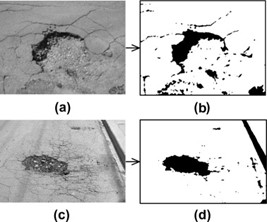
\includegraphics[width=0.4\textwidth]{img/abra1.jpg} 
	\caption{Kátyún belüli árnyékok szemléltetése \cite{abed_analysis_2023}}
	\label{fig:katyu_arnyék}
\end{figure}

A kátyún belüli árnyék mértékét és kontrasztját leginkább a fényforrás
iránya, azaz beesési szöge határozza meg, illetve a kamera
perspektívája, ezek a jelenségek jól megfigyelhetőek az
\ref{fig:katyu_arnyék}. ábra b és d részén. Jól látható,
hogy a d képen a fekete folt maga a teljes kátyú, míg a b képről ez nem
mondható el. A b képen csak a kátyú egy bizonyos része árnyékos így nem
fedi le a kátyú teljes területét. Ebből kifolyólag a fekete foltokon
további geometriai vizsgálatokat végeznek a bináris képeken, hogy
megállapítsák azt, hogy melyik esettel állnak szembe (b vagy d) az adott
képnél.

A vizsgálat lépései kiszámolják a folt súlypontját majd megnézik, hogy a
súlypont a folton belül van e, ezzel megállapítják, hogy az alakzat
tömör vagy kifli alakú. Abban az esetben, ha tömör, de nyújtott vagy
kifli alakú, akkor megnézik, hogy mennyire hosszúkás és mennyire vékony
a vonal. Ehhez excentricitását, leghosszabb átmérőt és területet
számolnak. Majd a következőként dönt, ha a súlypont kívül van vagy a
forma hosszúkás és vékony akkor az árnyék nem fedi le a kátyú teljes
területét. Ellenkező esetben, ha a súlypont belül van, és a forma nem
extrém módon hosszúkás, és se nem vékony, akkor az sötét folt a teljes
kátyút jelöli.

Következik a textúra elemzése, itt igyekeznek megkülönböztetni a valódi
kátyúkat a többi sötét és nagyjából ellipszis alakú foltoktól (például:
olajfolt, sima árnyék, egyéb objektum). Ennek meghatározása érdekében a
foltok belsejét és a külsejét vizsgálják. Ezt úgy érik el, hogy veszik a
bináris képet, majd kiterjesztik morfológiai dilatáció segítségével. Ez
azért kell, hogy a lehetséges kátyú közvetlen szélén lévő, bizonytalan
pixelek ne számítsanak bele a külső régióba. Az eredeti bináris képből
kivonják ezt a kiterjesztett képet, ezentúl kivonják belőle, magának a
vizsgált foltnak a területét is. Ami megmarad az lesz a megbízható,
referenciaként felhasználható, ép út textúrája.

Az ötlet az, hogy a kátyú belseje általában érdesebb, mint a sima út.
Megnézik az összes pixel szürkeárnyalatos intenzitás értékét az adott
folt belsejiben és kiszámolják ezeknek az értékeknek a szórását. A folt
területe sima, ha az intenzitások szórása alacsony, érdes, ha a szórás
magas. Mivel a kátyú szemcsés ezért spot filter-eket (folt szűrő)
használnak az eredeti szürkeárnyalatos képen. Ezek a szűrők az ilyen
apró, pontszerű vagy foltszerű mintázatokat találják meg a képen belül.

Összehasonlítás, mindkét folt régióhoz (belső és külső) létrehoznak egy
egy 5 dimenziós jellemzővektort. Ennek az 5 eleme a következő,
szürkeárnyalati szórás, és a cikkben használt 4db spot filter válaszának
szórása. Kiszámolják mindkét vektor hosszát. A vektor hossza itt azt
méri, hogy összességében mennyire erős a textúra az adott régióban az 5
mért jellemző alapján. Ha az adott folt belső vektorának a hossza
nagyobb, mint a külsőé akkor a belső textúra kátyút jelöl. Ellenkező
esetben nem tekinthető kátyúnak az adott folt. \cite{koch_pothole_2011}

A cikkben leírt módszer fő előnye, hogy textúra összehasonlítást
alkalmaz a hamis pozitívumok (pl. olajfoltok, árnyékok) hatékony
kiszűrésére, amivel figyelemre méltó, „86\%-os pontosságot ér el''
klasszikus képfeldolgozó módszerként \cite{koch_pothole_2011}. A cikk nem közöl konkrét
futási időt, de a többlépcsős képfeldolgozási folyamatok miatt, szinte
biztos, hogy magas számítási idővel járnak, így egy az egyben nem
használható valós idejű kátyú detektálásra. A szegmentálás
eredményessége erősen függ a fényviszonyoktól. A szerzők maguk is
elismerik, hogy olyan körülmények között, ahol minimális az árnyék (pl.
a nap magasan, merőlegesen süt), a módszer hibázhat \cite{koch_pothole_2011}. A módszer
nem adaptív, így valós idejű rendszer esetén nem alkalmazható ugyanis
több kritikus paramétert is használnak, amelyeket „manuálisan kellett
beállítani egy 50 képből álló tanító adathalmazon'' \cite{koch_pothole_2011}.

\subsubsection{Pothole Detection with Image Processing and Spectral
	Clustering}

Emir Buza, Alvin Huseinovic és Samir Omanovic egy spektrális
klaszterezéses megoldást javasoltak 2013-ban.

Első lépésben klasszikus hisztogram alapú küszöbölést végeznek a képen,
az RGB képet szürkeárnyalatos képpé alakítják, majd a hisztogramon Otsu
féle küszöbölés alkalmaznak. A végeredmény egy bináris kép lesz,
mégpedig úgy, ha az adott pixel kisebb vagy egyenlő a küszöb értékkel(T)
akkor objektum, azaz 1, ha az adott pixel nagyobb, mint T akkor háttér,
azaz 0. Látható, hogy a \ref{fig:zajos_binaris}. ábra zajos
és a kátyún túl a repedések, árnyékok és egyéb vonalak is feketék.\cite{buza_pothole_2013}

\begin{figure}[htbp]
	\centering
	\begin{minipage}{0.4\textwidth}
		\centering
		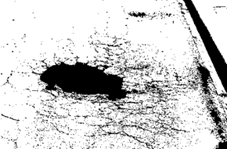
\includegraphics[width=\linewidth]{img/abra2_1.png}
		\caption{Zajos bináris kép \protect\cite{miller_distress_2014}}
		\label{fig:zajos_binaris}
	\end{minipage}\hfill
	\begin{minipage}{0.4\textwidth}
		\centering
		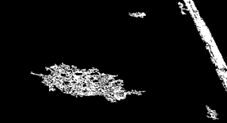
\includegraphics[width=\linewidth]{img/abra2_2.png}
		\caption{Szűrt bináris kép \protect\cite{miller_distress_2014}}
		\label{fig:szurt_binaris}
	\end{minipage}
\end{figure}

Ezért a cikk szerzői sajátos megoldást dolgoztak ki, aminek az eredménye
a másik \ref{fig:szurt_binaris}. ábrán látható.
Bevezettek egy deltaváltozót, amit úgy számítottak ki, hogy az Otsu
küszöbértékből kivonták a kép átlagos intenzitását, majd ennek az
abszolút értékét kettővel megszorozták. A delta értéket arra használták,
hogy az eredeti szürkeárnyalatos képből két új vágott képet hozzanak
létre. Az eredeti kép aljáról delta sort vágnak le, ez lett az egyik
vágott kép, aztán eredeti képnek a tetejéről vágtak le delta sort, ez
lett a másik. Majd ebből a két vágott kép különbségéből határozták meg a
bináris képet. Az eredmény sokkal tisztább, jobban kiemeli a kátyút, és
a zajok nagyrészét kiszűrte a képről. A
\ref{fig:zajos_binaris}. ábra jól rámutat, hogy a kátyú
mellett leginkább egyenes vonalak maradtak meg. Ezeket excentricitás
módszer segítségével távolítják el, amit ismertettem a \nameref{pothole-detection-in-asphalt-pavement-images} című alfejezetben a
\pageref{pothole-detection-in-asphalt-pavement-images}.oldalon.Továbbá
a nagyon apró régiókat, alakzatokat is törlik, végül minden olyan
alakzatot törölnek, ami hozzá ér a kép széléhez. Így kapnak egy szűrt
csak a kátyút tartalmazó bináris képet.

A cikkben ezzel párhuzamosan elvégzik az eredeti szürkeárnyalatos kép
hisztogramján a spektrális klaszterezést. A klaszterezés lényege, hogy a
hasonló előfordulású intenzitásokat egy csoportba gyűjtsék ki, így
létrejön k-db csoport, klaszter. A hasonlósági vizsgálatot Gauss
kernellel teszik, a hisztogram intenzitások(0-255ig) gyakoriságát
hasonlítják össze az egyenlet segítségével, az így kapott étékeket a
hasonlósági mátrixban tárolják el. Aztán fokszám majd Laplace mátrixot
számolnak, a fokszám mátrix esetén végig iterálnak a hasonlósági mátrix
sorain, és szummázzak azokat ezzel egyfajta összegzett népszerűség
értéket rendelnek az intenzitásokhoz. Majd egy új mátrix főátlóiba
beírják ezeket a népszerűség értékeket. Laplace mátrix számítása, a
fokszám mátrixból kivonják a hasonlósági mátrixot, az így kapott
256×256-os mátrix főátlója az intenzitások fokszámait, míg a többi elem
a gráf szerkezetét írja le. Ezután ennek a Laplace mátrixnak elvégzik az
eigen-decomposition-t (sajátérték-felbontását), ami kiszámítja a
sajátértékeket. A cikkben említett algoritmus 1 ezeket sajátértékeket
használja fel, hogy automatikusan meghatározza a klaszterek számát (k).

Végezetül, a tisztított bináris képet, valamint az eredeti
szürkeárnyalatos kép klaszterezéséből kapott eredményt felhasználva, az
algoritmus 2-őt futtatják, ami seed points-okat (mag pontokat) hoz
létre, ezekkel a pontokkal összekapcsolja a kétféleképpen feldolgozott
képet. A \ref{fig:modszer_vegeredmenye}. ábra szemlélteti, a mag
pontokat és az összekapcsolt végeredményt. \cite{buza_pothole_2013}

\begin{figure}[htbp]
	\centering
	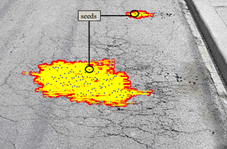
\includegraphics[width=0.4\textwidth]{img/abra3.png}
	\caption{A cikkben bemutatott módszer végeredménye \protect\cite{miller_distress_2014}}
	\label{fig:modszer_vegeredmenye}
\end{figure}

A cikkben leírt módszer fő előnye, hogy egy olcsó, felügyelet nélküli
eljárás, amely nem igényel drága berendezéseket vagy külön tanítási
fázist. A spektrális klaszterezés alkalmazásával a tesztadatbázison
„81\%-os pontosságot'' értek el, ezen felül „rough estimation'' (durva
becslést) adtak a kátyúk területére \cite{buza_pothole_2013}. Ilyesfajta durva becslés
jól jöhet a későbbiekben, amikor a kátyú méretét és elhelyezkedését
fogom vizsgálni. Hátránya azonban, hogy ez a becslés valóban csak
közelítő, mivel a végső területet egy egyszerű téglalap alapján számolja
ki, de viszonyítási alapnak jó lehet. A cikk nem tárgyalja a valós idejű
feldolgozást, ami részben érthető, hiszen a hibás képkockák kiválasztása
manuálisan végzik. Bár a teszteléshez használt hardver alapján „Intel
Core2 2.80GHz CPU és 4GB RAM'' a valós idejűség akkoriban nem volt
reális cél, modern számítási kapacitással ez ma már megoldható lenne
\cite{buza_pothole_2013}. A valós idejű működés eléréséhez azonban elengedhetetlen a
teljes folyamat automatizálása, kezdve egy olyan algoritmussal, amely
képes a videófolyamból pontosan, emberi beavatkozás nélkül kiszűrni a
releváns, hibát(kátyút) tartalmazó képkockákat.

\subsubsection{\texorpdfstring{Pothole detection on asphalt pavements from
		2D-colour pothole images using fuzzy \emph{c}-means clustering and
		morphological
		reconstruction}{Pothole detection on asphalt pavements from 2D-colour pothole images using fuzzy c-means clustering and morphological reconstruction}}

Ouma és Hahn 2017-ben egy többlépcsős, hibrid algoritmust dolgoztak ki.
Ennek oka, hogy úgy vélték a 2D képfeldolgozó módszereknek alapvető
korlátai vannak kátyúdetektálás terén. Különösen kiemelték, hogy a
széles körben alkalmazott küszöbölési eljárások gyakran érzékenyek a
változó fényviszonyokra és az útburkolat textúrájának inhomogenitásaira.
Ezek a tényezők rossz irányba befolyásolják a szegmentálás kimenetét.
Illetve, a hagyományos, "kemény" szegmentálási módszerek
rugalmatlanságáról esett szó a cikkben, amelyek a kép minden egyes
pixelét egyértelműen és kizárólagosan besorolják egyetlen kategóriába.

A javasolt megoldásban az első lépés a zajszűrés és a szegmentációhoz
használatos küszöbérték megtalálás áll. Ehhez A wavelet transzformációt
használnak, a fő előnye, hogy több skálán elemzi a képet egyszerre,
ellentétben a hagyományos szűrőkkel. Azaz képes a kép finomabb és
durvább részleteit külön kezelni. Ezáltal a zaj jelentős részét
eltünteti miközben a fontos jellemzőket jobban megtartja. Cikkben a
Daubechies waveletet-et használnak, felbontják a képet különböző
szintekre, szétválasztva a durvább, kisebb felbontású pixel
információkat, és a magasabb, finomabb, részletinformációkat. Ezt
követően a részlet koefficienseken "lágy" küszöbölést végeznek, amely a
zajnak tulajdonított kis értékű koefficienseket nullázza vagy csökkenti,
miközben a fontosabbakat megőrzi. Végül az inverz wavelet
transzformációt segítségével a módosított koefficiensekből
visszaállítják a képet, amely így egy simított, zajcsökkentett lesz.

Klaszterezés lépésben a Fuzzy c-means clustering-et használják a
szerzők. Mert így bizonyos pixeleket egyszerre több kalszterben is
számon tudnak tartani százalékos arányba kifejezve (például egy pixel
70\%-ban kátyú, 30\%-ban út). Az algoritmus véletlenszerű kezdeti
klaszterközéppontokból indul ki majd felváltva frissíti a pixelek
tagsági fokait a középpontoktól való távolság alapján. Aztán újra
számolja a klaszterközéppontokat a pixelek tagsági fokokkal súlyozott
átlagaként, amíg a tagsági fokok változása egy küszöbérték alá nem esik.
Ez a folyamat a költségfüggvényt minimalizálja, amely a pixelek és a
hozzájuk tartozó klaszterközéppontok közötti, tagsági fokokkal súlyozott
távolságok összegét méri.

Utolsó lépésben a morfológiai rekonstrukciót hajtanak végre, amely
pontosítja a kalszterezést. Két képet használ: egy marker képet, ami a
klaszterezés során azonosított potenciális kátyú pixeleket tartalmazza,
és egy maszk képet, ami az eredeti wavelet-szűrt kép intenzitásait
használja, felső korlátként. A két bement alapján újra felépíti a képet
a markerek alapján, de csak azokat a részeit tartja meg, amelyeket a
maszk "megenged". \cite{ouma_pothole_2017}

Ez a hibrid módszer kecsegtető és érdekes részekből épül fel. Az elért
„87.5\%-os átlagos pontosság'' és az hogy nem igényel tanító adatbázist,
nagyon jó eredmény \cite{ouma_pothole_2017}. Ugyanakkor jelentős hátrányai is vannak,
amelyek korlátozzák a gyakorlati alkalmazhatóságát. A legkritikusabb
probléma a rendkívül lassú, „95 másodperces átlagos futási idő
képenként'', ami teljesen kizárja, hogy egy az egyben fel tudjam
használni ezt a megvalósítást \cite{ouma_pothole_2017}. Bár figyelembe véve a szűrés
részletességét, a klaszterezést, majd pedig az iteratív morfológiai
rekonstrukciót, ez érthető futási idő még hardvertől függetlenül is. Az
a baj ezzel a megoldással, hogy a Fuzzy c-means clustering-et megelőzően
nagyon pontos szűrésre van szükség, ami viszont számításigényes. Ha
pedig nem megfelelő a szűrés akkor a szegmentálás nem lesz megfelelő.
Tehát csak a morfológiai rekonstrukción lehetne drasztikusan
változtatni, ám azt nem hiszem, hogy olyan sokat számítana, és hirtelen
valós időben futtathatóvá válna a program.

\subsubsection{Watershed-alapú valós idejű képfeldolgozás aszfaltúton található többszörös kátyúk észlelésére}
\label{watershed-alapu}

Tran Duc Chung és M. K. A. Ahamed Khan olyan valós idejű megvalósítást
javasolnak 2019-ben, ahol a feldolgozás egyszerűsége és a feldolgozási
ideje áll a középpontban. Ezt úgy érik el, hogy vesznek egy RGB (red
(vörös), green (zöld) és blue (kék)) képet, ezt szűrek árnyalatos képpé
konvertálják majd kijelölnek egy ROI (Range of Interest (érdekes
régió))-t a képen belül, amit vizsgálni fognak. Ezt követően csak a
ROI-val fognak számításokat végezni, ezzel csökkentve a számítási
kapacitást és időt. A ROI-n belül bináris és Otsu féle küszöbölést
alkalmaznak, hogy a szegmentálást, azaz a hátteret az objektumtól el
tudják jól különíteni. Következik a zajszűrés a ROI-n majd a megmaradt
összefüggő objektumok kiemelése dilatációval, erre két külön kernelt
használnak. A dilatációval eltűnnek a fekete (háttér) szigetek a ROI-n
belül és csak azok maradnak feketék, amik biztosan a hátteret képzik.
Ezt követően távolságtranszformációt~hajtanak végre a markerek (jelölők)
kiszámításához. A távolságtranszformációval minden egyes fehér pixelre
kiszámolják, hogy milyen távol van a legközelebbi fekete pixeltől ezzel
minden fehér pixelnek egy magasságot ad. Ezzel a módszerrel
meghatározhatóak olyan markerek, mint biztos háttér és biztos előtér
(objektum), illetve ismeretlen régió. Végül a marker térképet
felhasználva az eredeti RGB képen meghívják a watershed (vízgyűjtő)
algoritmus, ami az ismeretlen régiókat elválasztja hátérré vagy
előtérré. \cite{chung_watershed-based_2019}

Nagyon inspirálónak tartom a ROI használatát, mert az általános, hogy a
képeken több út (háttér) szerepel, mint kátyú (objektum), ROI
meghatározással sok felesleges számítást lehet megspórolni. A cikkben
vannak pontos mérési adatok FPS (Frames Per Second (képkocka
másodpercenként))-ben megadva, ebből az vonható le következtésként, hogy
minél több kátyú vagy kátyú részlet van a képen, annál rosszabb a
feldolgozás sebessége, legrosszabb mérés 26,4 FPS a legjobb pedig 37,4
FPS \cite{safyari_review_2024}. A „képek 640×480 pixel felbontásúak'' voltak és az
„algoritmus Intel Core i5 5255u processzorral és 4GB DDR3 memóriával
ellátott számítógép futatta, 1600 MHz-es buszon'', GPU-t nem
említenek \cite{chung_watershed-based_2019}. Itt felmerült bennem az a lehetőség, hogy GPU
segítségével lehetne gyorsítani azokat az eseteket, amikor több kátyú
van egyszerre a képen. Kátyú száma ROI kellene létrehozni, és azok
párhuzamosan GPU-n vagy akár CPU-n is futhatnának. A 30 FPS és a feletti
teljesítmény meglehetősen jónak mondható és már tényleg valós idejű
rendszerként használható lehet.

Pontoságról nem esik szó a cikkben, de feltételezhető, hogy minden úton
lévő nagyobb objektumot hasonlóan detektál gondolok itt árnyékra,
felfestésre, foltokra tehát nem csak kátyúkat.

Még az Otsu féle statisztikai technikára térnék ki, mert jó minőségű
képeken, amin kevés zaj van azokon a küszöbérték meghatározása jó
működik jellemzően ilyenek voltak a példaképek a cikkben. Az objektum
mérete, az objektum helyzete és gyengébb, zajos képminőség befolyásolja
a teljesítményt és előfeldolgozást kell végezni a képen a jó végeredmény
érdekében. \cite{goh_performance_2018}
%%%%%%%%%%%%%%%%%%%%%%%%%%%%%%%%%%%%%%%%%%%%%%%%%%%%%%%%%%%%%%%%%%%%%%%%%%%%%%%%%%%%%%%%%%%%%%%%%%%%%%%%%%%%%%%%%%%%%%%%%%%%%%%%%%%%%%%%%%%%%%%%%%%%%%%%%%%%%%%%%%%%%%%%%%%%%%%%%%%%%%%%%%%%%%%%%%%%%%%%%%%%%%%%%%%%%%%%%%%%%%%%%%%%%%%%%%%%%%%%%%%%%%%%%%%%%%%%%%%%%%%%%%%%%%%%%
\subsection{Konvolúciós neurális hálózatokon alapuló úthibadetektálás}

Az előző
\nameref{klasszikus-kepfeldolgozason-alapulo-uthibadetektálas} című fejezetben,
általam bemutatott algoritmusok „műveleteket hajtanak végre a bemeneti
képeken, hogy hasznos információkat nyerjenek ki belőlük'' \cite{r_comprehensive_2022}.
Ezek a képfeldolgozó algoritmusok, több egymásra épülő merev lépésekből
állnak (előfeldolgozás, szegmentálás, jellemzőkinyerés, osztályozás).
Bár a teljesítményük 90\% körül mozog, de a számítási idő magasnak
mondható, főleg valós idejű rendszerhez viszonyítva. Továbbá, a
klasszikus módszerek implementálása során a paramétereket (például:
szűrőméretek, küszöbértékek) manuálisan finom hangoljak, hogy az adott
bemeneti adathalmazon optimális megoldás elérése érdekében. Ennek
következménye az alacsony robusztusság, mivel a végeredmény túlságosan
érzékennyé válik a bemeneti adatok specifikus jellemzőire, és az azokhoz
igazított paraméterekre. Ez a megközelítés működőképes, de inkább
homogén környezetben (például: gyártósori minőségellenőrzés), míg az
inhomogén esetekben, mint az úthibák, kátyúk detektálása, ahol az út
felülete és a fényviszonyok képkockáról képkockára változhatnak, nem
beszélve a kátyúk eltérő tulajdonságairól, ez a módszer nem bizonyul
járható útnak számomra.

Deep learning (mélytanulás) a mesterséges intelligencia egyik
kulcsfontosságú és napjainkban divatos részhalmaza. Ezen a területen
belül a convolutional neural network (CNN, konvolúciós neurális hálózat)
jelentik azt a specializált architektúrát, amelyet kifejezetten a
képekhez hasonló, rácsszerkezetű adatok feldolgozására és elemzésére
fejlesztettek ki. A hálózat három rétegből tevődik össze, konvolúciós
réteg, ami a bementi kép vagy a future map (jellemző térkép) pixel
értékein halad végig egy vagy több kernel-lel (filter, csúszó ablak) és
elvégzi a konvolúció műveletet. Az így létrejött jellemző tértkép(ek) a
csúszó ablak(ok) által kiemelt tulajdonságokat tartalmazza. Ezt követően
a pooling layer (tömörítő réteg) a jellemző térképen szereplő
tulajdonságokat felerősíti, és tovább csökkenti a dimenzióméretet.
Harmadik a fully connected layer (teljesen összekapcsolt réteg) a képek
osztályozást végzi. Az aktivációs függvények teszik képessé a hálózatot
arra, hogy az adathalmazban rejlő komplex, nem lineáris mintákat,
összefüggéseket felismerjék. A csúszó ablakként funkcionáló konvolúciós
kernelek súlyparamétereit a hálózat a tanítási folyamat során (például:
backpropagation) finom hangolja. Ez az optimalizálás biztosítja, hogy a
hálózat által kinyert jellemzők a kívánt osztályozási eredményhez
vezessenek, minimalizálva a hibát a tanító adathalmazon. \cite{r_comprehensive_2022}

A konvolúciós neurális hálózatokon belül három számítógépes látása
feladat típust különböztetünk meg, image classification (kép
osztályozás), object detection (objektum detektálás) és semantic
segmentation (szemantikus szegmentálás) \cite{r_comprehensive_2022}. A kép osztályozás
esetén a kimenet egy címke lesz, például a kép tartalmaz kátyút, vagy a
kép nem tartalmaz kátyút. Tehát ebben az esetben a képen szereplő kátyúk
darabszámáról, és a betöltött pozíciójukról, sem ad információt. Az
objektum detektálás estén ez nincs így, itt a kimenet mind egyes kátyú
köré bounding box-ot rajzol, ezzel az összes kátyút és azok pozícióját
is jelöli a képen. A szemantikus szegmentálás szolgáltatja a
legrészletesebb információt a képről, minden egyes pixelhez címkét
rendel. Kijelenthető, hogy jelenleg valós idejű kátyú detektálásra, az
objektum detektálás típus használható a legjobban, ezért a továbbiakban
csak ezeket fogom részletezni. \cite{ma_computer_2022}

\subsubsection{Kétfázisú objektumdetektálás Faster
	R-CNN}

2016 január 6.-án Shaoqing Ren, Kaiming He, Ross Girshick, és Jian Sun
publikálták a Faster R-CNN: Towards Real-Time Object Detection with
Region Proposal Networks című folyóiratcikket. Abban az időben a legjobb
objektumdetektáló algoritmusok a Region-based CNN (R-CNN) családba
tartoztak. A korábbi verziók (R-CNN, Fast R-CNN) pontossága már nagyon
jónak számított, de a sebességükről ugyan ez nem volt elmondható.
Működésük, első lépéseként egy külső region proposals (régiójavaslatok)
algoritmus több potenciális bounding box-ot generál. Ezt követően a
rendszer egy konvolúciós neurális hálózatot futtat le minden egyes
javasolt régión, hogy azokból features (jellemzőket) nyerjenek ki,
amelyeket aztán egy különálló osztályozó értékel. A szerzők a sebességen
akartak változtatni, a szűk keresztmetszetet a régiójavaslatok
jelentették. A régiójavaslatok meghatározásához klasszikus képfeldolgozó
algoritmusokat használtak (selective search, edge boxes). A probléma az
volt, hogy a javaslatok generálása sokszor annyi ideig tartott, mint
maga az objektum detektáló hálózat. A cikk fő áttörése, hogy egy kicsi,
gyors neurális hálózattal, Region Proposal Network-el (RPN) hajtják
végre a régiójavaslatok generálását.

A következő \ref{fig:faster_rcnn_felepites}. ábra rámutat, hogy a
szerzők által leírt RPN jelentőségére, és, hogy miért nevezhető
two-stage-nek (két fázisú) az összes R-CNN-en alapuló implementáció.
Első fázis a régiójavaslatokért felelős, ez az, amit a RPN hálózat hajt
végre. Egyetlen feladata, hogy a teljes feature map-et (jellemzőtérkép)
gyorsan végig pásztázza, és olyan régió dobozokat javasol, ahol
valószínűleg valamilyen objektum található. Ez a fázis nem mondja meg,
hogy pontosan mi van abban a régió dobozban, csak azt, hogy ezeken a
területeket érdemes tovább vizsgálódni. Ezt követi a második fázis, ez
maga a detektálásért felelős, classifier modul. A RoI pooling elvégzi az
összevonást, RPN hálózat által tett javaslatokon és az azokhoz tartozó
jellemzőtérkép részleteken, majd az összevonást követően megkezdődik az
osztályozást. Eldönti, hogy a dobozban kátyú, autó vagy háttér van.
Továbbá, finom hangolja a dobozok koordinátáit, hogy az jobban
illeszkedjen az objektumra. Tehát a folyamat két egymásra épülő lépéből
áll, első a javaslat, második az osztályozás, ezért hívják kétfázisú
detektornak. \cite{ren_faster_2017}

\begin{figure}[htbp]
	\centering
	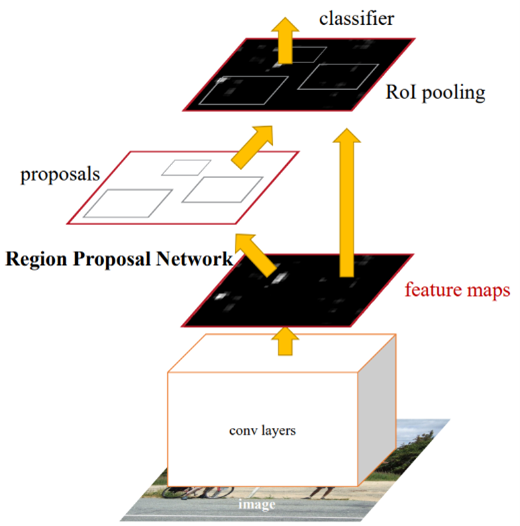
\includegraphics[width=0.4\textwidth]{img/abra4.png} 
	\caption{Faster R-CNN felépítése \protect\cite{ren_faster_2017}}
	\label{fig:faster_rcnn_felepites}
\end{figure}

Fontos, hogy itt a RPN nem a nyers bementi képen, hanem a törzs
kimentén, azaz a konvolúciós rétegek végső, mély jellemzőtérképén
dolgozik. Az RPN a cikkben egy 3×3-as csúszó ablakkal dolgozza fel a
jellemzőtérképet. A jellemzőtérkép minden egyes pozíciójában k darab
különböző méretű (például: kicsi, közepes, nagy), előre definiált anchor
box (horgonydoboz, referencia dobozt) használ. Ezek a dobozok, keretek
ugyanott vannak központosítva. Tehát a referencia doboz a 3×3-as csúszó
ablak középpontjához vannak társítva, de különböző méretekkel és
oldalarányokkal rendelkeznek. Majd a kimenetet egy alacsonyabb
dimenziójú vektorrá alakítják. Ezt követően, párhuzamosan két fully
connected layer (teljesen összekötött réteg) bemenetére adják ezt a
kilapított vektort. Az egyik az objectness score valószínűséget jósolja,
azaz, hogy az adott helyen van e bármilyen objektum, vagy csak háttér
található azon a területen. Másik a megfelelő horgonydobozt próbálja
kiválasztani az objektumhoz.

A Faster R-CNN legfőbb előnye a korábbi kétfázisú detektorokhoz (mint az
R-CNN vagy Fast R-CNN) képest elért drámai sebességnövekedés, amellyel
megközelíti a valós idejű működést (5-17 FPS). Bár a
\nameref{watershed-alapu} című alfejezetben a
\pageref{watershed-alapu}. oldalon 
ismertette watershed-alapú implementáció jobb, 30 FPS
sebességgel működik. A Faster R-CNN kiváló pontossággal detektálja az
objektumokat, mivel az RPN jobb minőségű javaslatokat ad, mint a fix
algoritmusok. A rendszer hátránya ugyanakkor a tanítási folyamat
bonyolultsága, a megosztott jellemzők optimalizálása a cikkben egy
komplex, 4 lépéses alternating training (váltott tanítási) sémát követ.
Habár általánosságban nézve gyorsnak számít, de ahogy a publikáció címe
is jelzi ez "csak" valós idejű megvalósítás felé vezető
megoldás. \cite{ren_faster_2017}

\subsubsection{Egyfázisú objektumdetektálás You Only Look Once v1}

2016 május 9.-én jelent meg a Joseph Redmon, Santosh Divvala, Ross
Girshick, Ali Farhadi közösen publikálták a You Only Look Once (YOLO)
Unified, Real-Time Object Detection (az első YOLO verzió). Fő szempont
az volt, hogy korábbi komplex, lassú és nehezen optimalizálható
megoldásoknál, gyorsabb architektúrát dolgozzanak ki, ami jobban tudja
utánozni az emberi vizuális rendszer, gyorsaságát és pontosságát.

A YOLO regressziós problémaként fogja fel a detektálást. Nincs szükség
komplex, többlépcsős folyamatokra. Egyetlen konvolúciós neurális
hálózatot használnak, és „a rendszernek csak egyszer kell ránéznie a
bementi képre, hogy prediktálni tudja a képen az objektumokat és a
hozzájuk tartozó pozíciót''. \cite{redmon_you_2016}

Első lépésben a bementi 448×448-as felbontású képet felosztja S×S méretű
grid-ekre (rácsokra, cellákra), ha egy objektum a középpontja belesik az
adott rácsba, akkor az a bizonyos rács felelős, annak az objektumnak a
detektálásáért. Fontos, hogy egy objektum átlóghat több különböző
cellába is, de a középpontja csak egy cellában lehet, és az a cella
felel azért az objektumért. A predikció során minden egyes objektum köré
bounding box-okat (határoló dobozokat) rajzolnak, azaz bekeretezi az
objektumok területeit a képen belül. Minden egyes határoló doboz az
alábbi értékekből épül fel, cellán belüli lokális x,y koordináták, amik
a detektált objektum középpontját írják le (ez a cella felel az
objektumért). Továbbá tartalmaz w,h globális koordinátákat a teljes
képhez képest, ezen információk alapján rajzolják ki a keretet az
objektum köré. Fontos megjegyezni, hogy x,y,w,h mind relatív értékek,
azaz 0-1 közöttiek így a tanítás kis számokkal zajlik. Minden
bekeretezett objektumokhoz még egy confidence score-t (megbízhatósági
pontszámot) rendel, amivel mérni tudják, hogy mennyire biztos a modell
abban, hogy a bekeretezett doboz tartalmaz objektumot és hogy mennyire
pontos a bekeretezése. Egy cellán belül B-db bounding box javaslat jön
létre, a javaslatok nem tudják, hogy pontosan mi az objektum (például:
kátyú vagy macska), csak az objektum létét és helyét becslik. Van C-db
osztály, amit detektálni akarnak, ehhez a cikkben a Pascal VOC
adathalmazt használják, amely 20 különböző osztályt tartalmaz (C = 20).
Minden egyes cellához a bounding box-októl függetlenül, C-db
valószínűséget számolnak a cella vizuális tartalma alapján. Tehát minden
egyes cellához tartozik egydarab 20 elemű one hot vector, ami
tartalmazza a cellához tartozó osztály valószínűségeket. Végül ezeket a
predikciókat egy tesorba (többdimenziós adattároló) helyezi, aminek a
dimenzió szám képlete a következő: \cite{redmon_you_2016}

„$S \times S \times (B \times 5 + C)$”\cite{redmon_you_2016}

Ez a tensor a hálózat feje, adja meg a hálózat végső kimenetét, a
cikkben B=2-vel (egy cellában két bounding box javaslat jön létre), de a
kimenetben egy cellához csak az egyik javaslatot tartják meg. Ennek
menet a következő, a cellához tartozó maximális C objektum
valószínűséget, össze szorozzák külön, külön mind a két javasolt
bounding box-hoz tartozó confidence score-ral, és a magasabb szorzat
eredmény dönt. Végül a relatív kimenti értékeket, abszolút pixel
koordinátákká kell visszaszámolni a kirajzoláshoz. Így áll elő, a
bementi 480×480-as képen, hogy hol és milyen objektumok találhatóak,
ezeket az objektumokat a pixel koordináták alapján bounding box-okkal
jelölik körbe, a kimeneti képen.

A teljes YOLO architektúra két részre osztható, backbone (törzs) és a
head (fej), előbbiekben szó volt a hálózat végső kimentéről ez a hálózat
fejéhez tartozik. A hálózat törzse 24 darab konvolúciós rétegből áll,
ezek a rétegek között pooling rétegek helyezkednek el a kép térbeli
méretének csökkentése érdekében. Az architektúrának a törzs része
felelős a képi információk kinyeréséért és azok megtanulásáért. Ezzel
szemben a fejrész kettő fully connected layer-ből áll, a bemente egy
kilapított one hot vector a kimenete pedig az előző bekezdésben
részletezett tensor. A fejrész felelős a végeredmény előállításáért a
kinyert jellemzők alapján. A YOLO egy egységes hálózat, amely a teljes
detektálási feladatot ellátja, de a hálózat betanítása két egymásra
épülő részből áll. Első a pretraining (előtanítás) ebben a fázisban a
hálózat 20 konvolúciós réteget, egy average pooling réteget. végül egy
fully connected réteget tartalmaz. A tanításhoz, az ImageNet adathalmazt
használják, a tanítás végén az alapvető képi, vizuális jellemzőket
megtanulja a hálózat, így képes lesz a képeket osztályozni. Ezután a
betanított törzs hálózatot átalakítják, hogy a képek klasszifikációján
túl, objektum detektálásra is képes legyen. Az előtanított 20
konvolúciós réteg után további 4 új, véletlenszerűen inicializált
konvolúciós réteget és 2 új, szintén véletlenszerűen inicializált fully
connected réteggel létrejön a YOLO architektúra. Míg az előtanítás
224×224-es bementi felbontású képeken zajlott, addig a detektáláshoz
részletesebb vizuális információra van szükség, ezért a tanítása
következő része 480×480-as növelt képeken folytatódik. Itt már a Pascal
VOC adathalmazt használják fel a tanításhoz, és egytelen komplex loss
function-t (hibafüggvényt) készítettek hozzá a szerzők. A tanítás során
azokat a cellák tartják fontosabbak, amik objektumot tartalmaznak, és
azok a cellák kevésbé fontosnak, amik nem tartalmaznak objektumot. Azért
lényeges ez, mert egy objektumot egy cella reprezentál (az a cella, ahol
az objektum közepe található) így általánosságban több olyan cella van,
ami nem tartalmaz objektumot. Ezen a logika mentén másképp kell
"büntetni" a cellákat tanulás során, ha azok felelősek egy objektum
detektálásáért, akkor 5 szeresére megnövelik a bounding box
koordinátáinak pontosságáért járó "büntetést", ha viszont csupán
hátteret tartalmaz az adott cella, akkor 0.5 szeresére csökkentik az
objektumot nem tartalmazó cella "büntetését". Így teremtenek egyensúlyt
a tanítás során az eltérő cellák és azok eltérő előfordulása között.

Összeségében a YOLO (You Only Look Once) egy forradalmian új,
egységesített objektumdetektálási megközelítés, amely szakított a
korábbi, lassú és többlépcsős (pl. R-CNN-féle) módszerekkel. Ennek az
egységes architektúrának a meghatározó előnye az extrém sebesség,
amellyel megteremtette a valós idejű objektum detektálást. További
előnye, hogy a hálózat a teljes képet látja, így globális kontextussal
dolgozik, ezért sokkal kevesebb téves pozitív (háttér) hibát vét, mint a
korábbi régió alapú módszerek, és jobban generalizál (általánosít). A
felsorolt tulajdonságok miatt nagy valószínűséggel ezt fogom használni a
kátyúk detektálásához. Ugyanakkor a módszer hátránya a pontosság terén
fellelhető, mivel a YOLO több lokalizációs hibát vét, és nehezebben
birkózik meg a kis méretű objektumok pontos helymeghatározásával. \cite{redmon_you_2016}

2016-óta számos YOLO verzió jelent meg, amelyek fejlesztése már nem
feltétlenül az előbb bemutatott első verzió szerzőihez kötődik, hanem
több különböző, független kutatócsoport, fejlesztő és cég (például az
Ultralytics) nevéhez. Ez a fajta fejlesztői sokszínűség párhuzamosan
zajlott a modellcsalád folyamatos architekturális evolúciójával. Míg a
korai verziók viszonylag egyszerű, elemekből építkeztek addig, az újabb
(mint a YOLOv4, v5, v7 vagy v8) már szignifikáns változtatásokon mentek
keresztül, beleértve a gerinc hálózatok (pl. CSPDarknet)
optimalizálását, a jellemző-aggregációt végző nyak modulok (pl. FPN,
PANet) bevezetését. Valamint az alapvető detektálási stratégia
módosulását, például a Faster R-CNN átvett anchor box, majd az
anchor-free (horgonymentes) megközelítések alkalmazását. Ezek az
újítások együttesen tették lehetővé a sebesség és a pontosság folyamatos
fejlődését \cite{terven_comprehensive_2023}, \cite{hussain_yolo-v1_2023}.

Minden egyes YOLO verziót bemutatása helyett, a következő fejezetben,
csak a feladatomhoz specifikusan kapcsolódó verziókra térek ki. Tehát
olyan valós idejű, ipari gyakorlatban használatos, erőforrás hatékony,
és alacsony számítási igényük verziókra, amelyeket korlátozott
erőforrású eszközökön is jó futási eredményt produkálnak.

\subsubsection{YOLO metrikák}
\label{yolo-metrikak}

Először az összehasonlítási alapot adó egységes metrikákat írom le, és
ezek mentén fogom összehasonlítani a YOLO verziókat. Van négy darab
alapmutató, amiből a különböző mérési metrikákat kell számolni. Ezek a
true positive (TP, pedálú: a modell kátyút jósol a kimeneten és valóban
van kátyú a képen, a bounding box is jó helyen van, IoU), false positive
(FP, pedálú: a modell kátyút jósol, de valóban nincs kátyú a képen, vagy
van kátyú a képen és a bounding box rossz helyen van). False negative
(FN, pedálú: a modell nem talál kátyút a képen, pedig van kátyú a képen
csak nem találta meg), true negative (TN, pedálú: nem talál kátyút a
képen mert valójában nincs is kátyú rajta) \cite{liu_deep_2019}.

Intersection over Union (IoU) ez felelős a hálózat által prediktált
bounding box lefedettségéért, azaz a kimenet mennyire van átfedésben a
tanító képhez (ezeken a képeken az objektumokat kézzel, ember által
bejelölt, határoló dobozok jelölik, Angol kifejezéssel élve "ground
truth"-nak nevezhetőek) képest. Képlet: IoU = két boundig box
metszetének a területe / két bounding box uniójának a területe, ha a
kimenet 0 akkor nincs átfedés, ha a kimenet 1 akkor tökéletes az
átfedés. Küszöbértéket kell meghatározni a IoU-hoz, ha a köszöneteknél
nagyobb eredményt ad az IoU képlet akkor az true positive kimenetnek
tekinthető, ellenkező esetben false pozitive-nak \cite{terven_comprehensive_2023}.

Precision (precízió, pontosság) a hálózat kimenetének a megbízhatóságát
méri, helyes kimenetek száma / összes kimenet száma, képlete: „P = TP /
(TP + FP)'' \cite{vinoth_lightweight_2024}.

Recall (felidézés, érzékenység) ez a metrika az alaposságot méri, mennyi
kátyút ismer fel a bemeneten, helyesen megtalált objektumok száma /
összes objektum a képen, képlet: „R = TP / (TP + FN)''\cite{vinoth_lightweight_2024}.

Average Precision (AP) a Recall-ból és a Precision-ból számítható
metrika, ha a precízió küszöbértékét alacsonyra állítjuk akkor sok
objektumot fog találni a képen, hátránya, hogy megnő a false pozitvok
száma. Ennek köszönhetően magas lesz az érzékenységi érték. Ellenkező
esetben, ha a precízió küszöbértékét magasra állítjuk, akkor csak azokat
az objektumokat észleli, amiben nagyon biztos, és sokat figyelmen kívül
fog hagyni, azaz alacsony lesz az érzékenység mutató. Tehát a Precision
és a Recall függenek egymástól és ez oda vissza igaz. Az a AP-t
objektumkategória specifikusan számolják külön, külön. Ehhez kirajzolják
a Precision-Recall görbét, majd a görbe alatti területet számolnak,
tanító adathalmaztól (Pascal VOC vagy Microsoft COCO) függően kicsit
eltérő lépésekkel.

Ezzel szemben a mean Average Precision (mAP) az összes objektumkategória
átlagát számítja ki, egyetlen számot ad vissza, amit a modell általános
teljesítményének tekintenek \cite{terven_comprehensive_2023}, \cite{liu_deep_2019}.

\subsubsection{YOLOv5, YOLOv8 és YOLOv10
	fejlődése}

Az előző \nameref{yolo-metrikak} pontra támaszkodva és a 
\cite{hussain_yolov5_2024}-forrás alapján hasonlítom össze a címben említett YOLO
verziókat. Ebben az összehasonlításban csak olyan verziókról, és azok
specifikus változatairól esik szó, amelyek kifejezetten erőforrás
hatékonyan tudnak működni, valós időben, „edge deployment'' \cite{hussain_yolov5_2024}
(peremhálózati eszköz, például: okostelefon, drón, autóba szerelt
vezérlőegység) környezetben.

A YOLOv5, YOLOv8 és YOLOv10 verziókon belül, megkülönbözettünk további
változatokat, mint nano(n), small(s), medium(m), large(l), extra
large(x). Ezek a megnevezések a modell méretére, és a hozzá tartozó
számítási igényére utalnak. Tehát minél nagyobb a modell, annál több
paramétert tartalmaz, ezáltal nagyobb számítási igénnyel rendelkezik,
megnő a futási idő, cserébe egyre jobb a modell általános teljesítménye
(mAP).

Az Ultralytics 2020-ban mutatta be a YOLOv5-öt, ami jelentős ugrást
hozott teljesítmény és a használhatóság terén is, így gyorsan nagy
népszerűségre tett szert. Az \ref{tab:yolov5}. táblázat
szemlélteti az egyes modell méretek közötti különbségeket. A méréseket a
Microsoft COCO adathalmazon végezték \cite{hussain_yolov5_2024}.

\begin{table}[htbp]
	\centering
	\caption{YOLOv5 verziók összehasonlítása \protect\cite{hussain_yolov5_2024}}
	\label{tab:yolov5}
	\vspace{0.2cm}
	
	\resizebox{\textwidth}{!}{%
		\begin{tabular}{|l|c|c|c|c|c|c|}
			\hline
			\textbf{Modell} & \textbf{Bemeneti kép mérete} & \textbf{AP} & \textbf{AP 50} & \textbf{CPU futási idő (ms)} & \textbf{Paraméter szám (M)} & \textbf{FLOPs (B)} \\
			\hline
			YOLOv5n & 640 & 28,0\% & 45,7\% & 45 & 1,9 & 4,5 \\
			\hline
			YOLOv5s & 640 & 37,4\% & 56,8\% & 98 & 7,2 & 16,5 \\
			\hline
			YOLOv5m & 640 & 45,4\% & 64,1\% & 224 & 21,2 & 49,0 \\
			\hline
			YOLOv5l & 640 & 49,0\% & 67,3\% & 430 & 46,5 & 109,1 \\
			\hline
			YOLOv5x & 640 & 50,7\% & 68,9\% & 766 & 86,7 & 205,7 \\
			\hline
		\end{tabular}%
	} 
\end{table}

Jól látható, hogy minél nagyobb a paraméterszám annál pontosabb a
rendszer. Illetve az is, hogy minél kisebb a paraméterszám annál jobb a
futási idő. Számomra a futás idő kritikusnak tekinthető, ezért olyan
kompromisszumot kell találnom, ahol kellő gyorsasághoz elfogadható
pontosság társul.

2023-ban megjelent a YOLOv8 ugyancsak az Ultralytics csapat által, ami a
YOLOv5 sikeres alapjaira épített, ennek a tovább fejlesztésnek az lett
az eredménye, hogy jobb átlagos teljesítmény mutatókkal rendelkezik,
mint elődjei \cite{hussain_yolov5_2024}. A modell gyorsítása mögött pedig az NVIDIA
TensorRT optimalizációs szoftver (SDK) áll. A TensorRT kifejezetten mély
neurális hálózatok optimalizálására fejlesztették ki, NVIDIA GPU-khoz.
Ezzel segítve azokat a valós idejű rendszerek működését, ahol a sebesség
és a teljesítmény rendkívül fontos. Ezt kvantálással érik el, a mély
neurális hálózatokat általában 32-bites lebegőpontos (FP32) formátumban
tanítják, a minél pontosabb végeredmény elérése érdekében. A tanítás
befejezte után hajtják végre a kvantálást INT8-ra, TensorRT SDK
segítségével az adott NVIDIA GPU-ra. Előnye, hogy a modell mérete a
negyedére csökken, ezáltal a sebességnövekedés extrémnek mondható,
cserébe viszont pontosság vesztés lép fel \cite{varun_improving_2020} , \cite{vina_optimizing_2025}. A
\ref{tab:yolov8_kvantalas}. táblázat mérési eredményei a teljesítmény
mellett, a GPU (NVIDIA A100) futás időbeli hatalmas különbségekre mutat
rá, itt is a Microsoft COCO adathalmazon.

 \begin{table}[htbp]
	     \centering
	     \caption{YOLOv8 és a kvantálás ereje \cite{hussain_yolov5_2024}}
	     \label{tab:yolov8_kvantalas}
	     \vspace{0.2cm}
	     \resizebox{\textwidth}{!}{%
	     \begin{tabular}{|l|c|c|c|c|c|}
		         \hline
		         \textbf{Modell} & \textbf{Bementi kép mérete} & \textbf{AP} & \textbf{CPU ONNX futás idő (ms)} & \textbf{A100 TensorRT futás idő (ms)} & \textbf{FLOPs (B)} \\
		         \hline
		         YOLOv8n & 640 & 37,3\% & 80,4 & 0,99 & 8,7 \\
		         \hline
		         YOLOv8s & 640 & 44,9\% & 128,4 & 1,20 & 28,6 \\
		         \hline
		         YOLOv8m & 640 & 50,2\% & 234,7 & 1,83 & 78,9 \\
		         \hline
		     \end{tabular}
		    }
	 \end{table}

Fontosnak tartom kiemelni, hogy a \ref{tab:yolov8_kvantalas}. 
táblázatban szereplő A100 TensorRT futás idő (ms) oszlop értékei, egy
csúcskategóriás hardveren produkált futásidőket mutatja. Az NVIDIA A100
Tensor Core GPU kifejezetten adatközpontok számára lettek fejlesztve,
hogy a mesterséges intelligencia modellek valós időben tudjanak
működni \cite{nvidia_nvidia_nodate}.

YOLOv10 2024-ben jelent meg, Tsinghua Egyetem kutatói álltal. A fő
újítása az objektumokhoz tartozó bounding box hozzárendelésben rejlik.
Korábbi YOLO verziók one-to-many hozzárendeléssel dolgoztak, azaz a
detektálás során egy objektumhoz több bounding box-ot prediktálnak, így
több visszajelzés keletkezik, amiből a tanulás során jobb AP érhető el.
Ennek az a hátránya, hogy a redundáns bounding box-ok közül ki kell
választani egyet, minden objektumhoz. Ezt egy utófeldolgozási lépéssel,
a Non-Maximum Suppression (NMS) algoritmussal oldják meg, ami lassítja a
működést. Ezzel szemben a one-to-one hazarendelés szigorúan egy bounding
box-ot rendel az objektumokhoz. Ennek előnye, hogy nem kell
utófeldolgozó NMS algoritmust használni, de a tanítás lassabbá, és
kevésbé pontossá válik. YOLOv10 ötvözi a one-to-one és a one-to-many
hozzárendelést, „Consistent Dual Assignments''\cite{wang_yolov10_2024} néven hivatkoznak
rá \cite{hussain_yolov5_2024}. Ennek az architektúrális változtatásnak a futás béli
előnyeit mutatja be a következő \ref{tab:yolov8_v10_comp}. táblázat.

 \begin{table}[htbp]
	     \centering
	     \caption{YOLOv8 és v10 összehasonlítása \cite{hussain_yolov5_2024}}
	     \label{tab:yolov8_v10_comp}
	     \vspace{0.2cm}
	     \resizebox{\textwidth}{!}{%
	     \begin{tabular}{|l|c|c|c|c|c|}
		         \hline
		         \textbf{Modell} & \textbf{Paraméter szám (M)} & \textbf{FLOPs (B)} & \textbf{AP} & \textbf{End-to-end futásidő (ms)} & \textbf{Futásidő (ms)} \\
		         \hline
		         YOLOv8n & 3,2 & 8,7 & 37,3\% & 6,16 & 1,77 \\
		         \hline
		         YOLOv10n & 2,3 & 6,7 & 39,5\% & 1,84 & 1,79 \\
		         \hline
		         YOLOv8s & 11,2 & 28,6 & 44,9\% & 7,07 & 2,33 \\
		         \hline
		         YOLOv10s & 7,2 & 21,6 & 46,8\% & 2,49 & 2,39 \\
		         \hline
		     \end{tabular}
		    }
	 \end{table}

A \ref{tab:yolov8_v10_comp}. táblázatban szereplő end-to-end futás
idő, a teljes végrehajtási időt mutatja meg, azaz a gyakorlati
detektálási időt. Míg a futás idő (ms) oszlop csak a neurális hálózat
számítását méri, ebből jól látható az utófeldolgozás időbeli plusz
költségének mértéke. A méréseket NVIDIA T4 GPU-n végezték FP16-os
kvantálással, a Microsoft COCO adathalmazon \cite{wang_yolov10_2024}. Ebből következik,
hogy eltérő mérési értékek szerepelnek, \ref{tab:yolov8_kvantalas}. táblázat és a \ref{tab:yolov8_v10_comp}. táblázat között, YOLOv8 verziók terén.

\subsubsection{Rendelkezésre álló nyílt adathalmazok és versenyek a
	témában}

A projektem adatkészlet kiválasztásának szempontrendszere a következő. A
fejlesztés fókuszában a valós idejű, járműbe szerelt dashcam (fedélzeti
kamera) videófolyamán alapuló kátyúdetektálás áll. Ebből adódóan olyan
adathalmazra van szükségem, amely kifejezetten ebből nézőpontból
rögzített, valós forgalmi szituációkat tartalmazó képekből áll.

A szakirodalomban elérhető számos, úthibákkal és autonóm vezetéssel
foglalkozó globális referenciabázis, azonban a feladat fókusza miatt
ezek jelentős része nem alkalmazható közvetlenül a céljaim eléréséhez.

Az útfenntartási gyakorlatban széles körben elterjedtek a speciális
mérőjárművekkel vagy drónokkal, top-down \textbf{(}felülnézetből)
rögzített adathalmazok, mint például a German Asphalt Pavement Distress
(GAPs) \cite{wang_yolov10_2024} vagy a Crack500 \cite{yang_feature_2020}. Ezek az adatbázisok kiemelkedő,
pixel szintű pontosságot nyújtanak az aszfalt textúrájának és
repedéseinek vizsgálatához. De a merőleges képeken nem tudom
felhasználni mert más perspektívából közelítik meg a problémát.

Az adathalmazok másik jelentős szegmensét az önvezető járművek számára
készített globális, nagy diverzitású (időjárás, napszak)
referenciabázisok adják, mint amilyen a Cityscapes \cite{cordts_cityscapes_2016} vagy a
BDD100K \cite{yu_bdd100k_2020}. Ezek az adathalmazok kiválóak a szemantikus
szegmentációra (például az útfelület, a sávok, a gyalogosok és a
járművek elkülönítésére). Ugyanakkor nem fókuszálnak a lokális
úthibákra: nem tartalmaznak dedikált, bounding box ellátott jelöléseket
kátyúkra vonatkozóan.

A projekthez leginkább illeszkedő, okostelefonos és fedélzeti kamerás
felvételekből építkező Road Damage Dataset (RDD) adathalmazokra, illetve
az ezekhez kapcsolódó globális versenyek (pl. ORDDC) eredményeire fogok
támaszkodik. \cite{arya_crowdsensing-based_2022}

Maeda és munkatársai a 2018-ban publikált kutatásukban a világon
elsőként hoztak létre egy olyan nagyméretű, publikus adathalmazt, amely
kifejezetten a mozgó járművekből, okostelefonnal vagy fedélzeti
kamerával rögzített úthibákra fókuszál. A közzétett adatbázis elsődleges
célja egy olyan egységes referenciabázis megteremtése volt a kutatók
számára, amely segítségével a különböző úthibákat detektáló algoritmusok
teljesítménye objektíven összehasonlíthatóvá váljék.

Az „adathalmaz összesen 9 053 darab, valós forgalmi szituációban készült
képet tartalmaz, amelyeken 15 435 útkárosodást jelöltek meg bounding
box-okkal''\cite{maeda_road_2018}. A szerzők a hibákat nyolc különböző osztályba
sorolták, egy hierarchikus rendszer alapján. A sérüléseket első lépésben
repedésekre és egyéb hibákra bontották. A repedéseket ezt követően
finomabb kategóriákra osztották tovább. Az egyéb károsodások kategóriája
a kátyúk mellett olyan specifikus problémákat is magában foglal, mint
például az útburkolati jelek kopása vagy elmosódása.

A publikációban a szerzők kiemelik, hogy a gépi látás és a
képfeldolgozás területén korábban egyetlen kutatás sem fedte le az
útkárosodások ilyen széles és részletes skáláját. A 600×600 pixel
felbontású felvételeket rendkívül változatos földrajzi helyszíneken és
eltérő időjárási körülmények között rögzítették, aminek köszönhetően az
adatkészlet kiemelkedően jól reprezentálja a valós, mindennapi vezetési
környezetet. \cite{maeda_road_2018}

A 2018-as kezdeményezést követően a technológia és az adatigény robbanás
szerűén megnőtt. Ennek a fejlődésnek a következő nagy mérföldkövét Arya
és kutatótársainak 2022-es munkája, a CRDDC (Crowdsensing-based Road
Damage Detection Challenge) nevű nemzetközi verseny, valamint az ehhez
kapcsolódó RDD2022 adathalmaz publikálása jelentette. A tanulmány
rámutat arra, hogy a korábbi rendszerekhez képest több kritikus ponton
is paradigmaváltás történt az úthiba-detektálásban.

A legszembe tűnőbb változás az adathalmaz mérete és földrajzi
diverzitása volt. Míg a 2018-as verzió kizárólag Japánra korlátozódott,
addig a 2022-es adatbázis már hat különböző ország (Japán, India,
Egyesült Államok, Csehország, Norvégia és Kína) úthálózatát fedi le. A
jelentősen kibővített adatkészlet több mint 47 000 valós forgalmi
szituációban rögzített képet és mintegy 55 000 bounding box-al ellátott
annotációt tartalmaz. Ez a nemzetközi kiterjesztés tudományos
szempontból elengedhetetlen volt ahhoz, hogy a modellek általánosító
képességét vizsgálni lehessen.

Egy másik jelentős változás a hibakategóriák egyszerűsítése és ipari
standardizálása volt. A 2018-as kutatásban használt, nyolc osztályt
tartalmazó és gyakran nehezen elkülöníthető kategóriákkal dolgozó
rendszert, egy sokkal letisztultabb, négy fő kategóriából álló
struktúrára cserélték. Ez az új D-kódos rendszer kizárólag a kritikusan
fontos strukturális hibákra fókuszál. A hosszirányú repedésekre (D00), a
keresztirányú repedésekre (D10), az aligátorrepedésekre (D20), valamint
a kátyúkra (D40). Az olyan kevésbé releváns kategóriákat, mint az
útburkolati jelek kopása vagy elmosódása, a hatékonyság érdekében
elhagyták.

Végül a tanulmány rávilágított egy egyértelmű technológiai
generációváltásra is. Míg az első kutatásoknál még a régebbi SSD (Single
Shot MultiBox Detector) architektúrák domináltak, a 2022-es nemzetközi
verseny eredményei empirikusan is bizonyították, hogy az egyfázisú
detektorok, kiemelten a modern YOLO (You Only Look Once) változatok
vették át a vezető szerepet. A YOLO modellek az RDD2022 adathalmazon
kimagasló pontosságot és robusztusságot mutattak, végleg ipari
sztenderddé válva a fedélzeti kamerás úthiba-detektálás
területén. \cite{arya_crowdsensing-based_2022}

A következő ORDDC\textquotesingle2024 kihíváson pontosan ugyanazt az
RDD2022 nevű adathalmazt használta, amelyet a CRDDC\textquotesingle2022
verseny során tettek közzé. A technológiai újítás a valós idejű működés
és a pontosság egyensúlyának megteremtése érdekében a 2024-es év
kiemelkedő technológiai trendjévé a tudáspárlat, valamint a könnyűsúlyú
neurális architektúrák alkalmazása vált. \cite{arya_orddc2024_2024}

\subsubsection{\texorpdfstring{ Transfer Learning és fine-tuning a
		gyakorlatban}{ Transfer Learning és fine-tuning a gyakorlatban}}

A gépi tanulás, és különösen a mélytanulás (deep learning) egyik
legnagyobb kihívása, hogy a modellek sikeres betanításához hatalmas
mennyiségű, címkézett adatra van szükség. Azonban a megfelelő méretű
adathalmazok összegyűjtése gyakran túlságosan drága, időigényes, vagy
egyszerűen kivitelezhetetlen feladat. Erre a problémára nyújt megoldást
a transfer learning (transzfertanulás). Aminek alapelve, hogy egy
korábban már megoldott feladat során megszerzett tudást egy új, de
kapcsolódó problémára alkalmaznak. A folyamat során a modell egy
úgynevezett source domain-ból (forrástartományból) származó
információkat, például egy hatalmas, általános képadatbázison betanított
hálózat súlyait emel át, egy target domain-ba (céltartományba), ezzel
drasztikusan csökkentve az új feladat adatigényét.\cite{zhuang_comprehensive_2021}

Yosinski és kutatótársai \cite{yosinski_how_2014} bizonyították, hogy a konvolúciós
neurális hálózatok (CNN) rétegei hierarchikusan, az általánostól a
specifikus felé haladva építik fel a vizuális tudásukat. A hálózat
legelső rétegei univerzális, úgynevezett general jellemzőket tanulnak
meg felismerni, mint például a színfoltok, élek, vonalak, sarkok. Ezek a
vizuális alapelemek szinte minden képi adathalmazban azonosak, így
könnyen átvihető más hálózatokra is. Ezzel szemben a hálózat mélyebb,
végső rétegei az eredeti feladatra erősen specifikus jellemzőket
detektálnak (például egy adott objektum osztályhoz tartozó jellemzőket).

Erre a megfigyelésre épül a fine-tuning (finomhangolás) technikája.
Ahelyett, hogy egy hálózatot a nulláról, véletlenszerűen inicializált
súlyokkal kezdenének el tanítani, egy nagy adathalmazon előtanított
modell súlyait emelik át kiindulásnak. A finomhangolás során a hálózat
első, általános vizuális jellemzőket felismerő rétegeinek súlyait
megtartják, rögzítik. Így csak az utolsó, feladatspecifikus rétegeket,
valamint az osztályozó réteget tanítják újra a saját, kisebb
adathalmazunkon. Ez a megközelítés lehetővé teszi a modell számára, hogy
a korábban rögzített álltalános jellemzőkre építve hozzáigazítsa a
specifikus rétegeket az új problémához. \cite{yosinski_how_2014}

A transzfertanulás és a finomhangolás együttes alkalmazásával drasztikus
előnyökre lehet szert tenni a nulláról történő betanítással szemben.
Zhuang és munkatársai \cite{zhuang_comprehensive_2021} alapján ez három fő teljesítménymutatóban
jelentkezik a tanulási görbén.

Magasabb kezdeti teljesítmény, mivel az előtanított modell már az első
tanítási lépések előtt felismeri a vizuális alapokat, a kezdeti
pontossága sokkal magasabb szintről indul, mint egy inicializálatlan
hálózaté.

Gyorsabb konvergencia, a finomhangolás során a hálózat meredekebb
tanulási görbét ír le, vagyis nagyságrendekkel kevesebb iteráció és
számítási idő alatt éri el az optimális pontosságot.

Legfontosabb hozadék a jobb végső teljesítmény, azaz a végső pontossága
szinte mindig felülmúlja a nulláról tanított modellekét, még abban az
esetben is, ha az utóbbiakat végtelen ideig próbálják tanítani a
rendelkezésre álló korlátozott adathalmazon.




\subsection{Detektált hibák lokalizálása}

A kátyúk magabiztos felismerését követően, ebben a szakaszban a
detektált úthibák pontosabb térbeli pozíciójának meghatározása a cél,
amely a képi információk valós világkoordinátákra történő leképezéssel
(image to world konverzió) valósítható meg. Jelen fejezet a geometriai
képalkotás elméleti hátterét, azt követően pedig a transzformációs
eljárásokat tárgyalja, amelyek lehetővé teszik a pixelkoordináták
fizikai távolsággá alakítását.

\subsubsection{Geometriai képalkotás elméleti háttere}

\subsubsection*{Lyukkamera modell}

Szeliski \cite{szeliski_computer_2011} munkája alapján a pinhole (lyukkamera) modell a 3D-s
tér és a 2D-s kép közötti leképzés legegyszerűbb geometriai leírása,
amelyben a fénysugarak egyetlen ponton, a vetítési középponton haladnak
át, lencsék alkalmazása nélkül. A modell matematikai alapját a hasonló
háromszögek képezik, amelyek segítségével a rendszer egy 3D-s pont (x,
y, z) koordinátáit a képsík (x, y) koordinátáira vetíti, ahol az
összefüggést a fókusztávolság (f) és a mélység (z) aránya határozza meg:
\("x = f \times \frac{x}{z}"\) és „\(y = f \times \frac{y}{z}"\). A
könyv részletezi, hogy a számítógépes látásban ezt a leképzést gyakran
homogén koordinátákkal és egy 3×4-es vetítési mátrixszal írják le, amely
szétválasztja a kamera belső paramétereit (mint a fókusztávolság és a
képközéppont eltolása) és a külső paramétereket (a kamera térbeli
pozícióját és orientációját). Bár a modell idealizált és nem számol a
lencsetorzításokkal vagy az elmosódással, Szeliski kiemeli, hogy ez
szolgál alapul a bonyolultabb képalkotási rendszerek megértéséhez és a
kamerakalibrációs eljárásokhoz is.

\subsubsection*{Inverz vetítés}

Szeliski könyve alapján a pixel-koordináták világ koordinátákká való
transzformációja, azaz az inverse projection (inverz vetítés) egy
eredendően többértelmű probléma, mivel a 3D tér 2D síkra történő
leképezése során a mélységi információ elvész. A szerző részletesen
kifejti, hogy a lyukkamera modell matematikai keretrendszerében egy
adott képpont visszavetítése, nem egyetlen konkrét térbeli pontot, hanem
a kamera vetítési középpontjából kiinduló, és a képponton áthaladó ray
sugarat határoz meg, a háromdimenziós térben. Ebből adódóan a pontos
világkoordináták (x, y, z) helyreállításához a kamera belső és külső
paramétereit tartalmazó vetítési mátrix inverzének alkalmazása önmagában
nem elegendő. A megoldáshoz ahogy Szeliski a geometriai képalkotásról
szóló fejezetekben tárgyalja elengedhetetlen valamilyen kiegészítő
geometriai felvetés, információ, például ismert mélység, több
nézőpontból származó háromszögelés vagy egy ismert síkkal, talajjal való
metszéspont meghatározása \cite{szeliski_computer_2011}.

\subsubsection*{Kamera kalibráció}

Richard Szeliski könyve alapján ismertetem a geometriai kamera
kalibráció folyamatát, amely a számítógépes látás egyik legalapvetőbb
lépése a 3D-s tér rekonstrukciójához \cite{szeliski_computer_2011}.

A geometriai kamera kalibráció az a folyamat, melynek során
meghatározzuk a kamera belső geometriai és optikai tulajdonságait,
valamint a térbeli helyzetét. A kalibráció elengedhetetlen minden olyan
alkalmazásnál, ahol a 2D-s képi információból pontos metrikus
következtetéseket kívánunk levonni a 3D-s valóságról. Nyers,
kalibrálatlan képek esetén ugyanis a lencsetorzítás és a vetítési
paraméterek ismeretének hiánya, lehetetlenné teszi a precíz
távolságbecslést vagy a képen szereplő tárgyak méretének meghatározását.

A kalibrációs modellt a lyukkamera modellre építi, amelyet a további
lépésekkel egészít ki. A szerző két lépést különít el a kalibrációs
folyamat során, belső paraméterek és külső paraméterek.

A belső paraméterek a kamera belső tulajdonságait írják le, amelyek
állandóak tekinthetőek. Ide tartozik a fókusztávolság, amely a nagyítás
mértékét határozza meg, valamint az optikai középpont, ahol az optikai
tengely metszi a képsíkot. Továbbá ki hangsúlyozza, hogy a valós
lencsék, különösen a nagylátószögűek, radiális torzítást okoznak (a
képek széle görbül), amivel a kalibráció során számolni kell.

Külső paraméterek a kamera világkoordináta rendszerhez viszonyított
helyzetét és orientációját írják le. Míg a belső paraméterek jellemzően
fixek, a külső paraméterek minden egyes kép készítésnél változhatnak, ha
a kamera mozog.

A gyakorlati kalibráció során ismert geometriájú kalibrációs mintákat
(leggyakrabban sakktáblát) használnak. Az eljárás lépései a következők,
első az adatgyűjtés, a kamera több különböző szögből készít képet a
mintáról. Következő lépés a jellemző pont detektálása, az algoritmus
azonosítja a minta jellegzetes pontjait (pl. a sakktábla sarkait) a
képeken. Az utolsó lépésbe paraméterbecslé és optimalizáció történik,
mivel a pontok valódi 3D koordinátái ismertek a mintán, és láthatóak
azok 2D vetülete a képen, az algoritmus egy optimalizációs eljárással
(például a legkisebb négyzetek módszerével vagy a Levenberg-Marquardt
algoritmussal), addig finomítja a kamera paramétereit, amíg a
reprojekciós hiba minimális nem lesz. Ez a hiba a mért képpontok és a
matematikai modell által visszavetített pontok közötti távolságot
jelenti, ennek minimalizálása garantálja a modell pontosságát.

Összességében a geometriai kamera kalibráció biztosítja azt a
matematikai transzformációt, amely lehetővé teszi, hogy a torzított,
perspektivikus 2D képekből visszanyerhető legyen a 3D-s tér
geometriailag helyes szerkezetét.

\subsubsection{Geometriai
	transzformációk}

\subsubsection*{Inverse perspective
	mapping}

Az inverse perspective mapping (IPM, inverz perspektív leképezés) egy
geometriai transzformáció, amelynek célja a kamera által rögzített képen
jelentkező perspektív hatás megszüntetése. Az IPM a kamera kép származó
információkat használja fel egy felülnézeti, „bird's eye view''
(madártávlati) kép létrehozásához, ahol a perspektívahatások nincsenek
jelen \cite{bertozz_stereo_1998}, \cite{oliveira_multimodal_2015}.

Alkalmazása ADAS rendszerekben és sávészlelés Az IPM kritikus szerepet
játszik az advanced driver assistance systems (ADAS, fejlett
vezetéstámogató rendszerek) előfeldolgozási fázisában, különösen a
sávfelismerés és sávtartás területén. A transzformáció legfőbb előnye,
hogy az új koordináta rendszerben a valóságban párhuzamos útburkolati
jelek (sávok) a képen is párhuzamosakká válnak, és állandó szélességűek
maradnak, függetlenül a távolságtól.

A módszer gyenge pontja a síkút feltételezés. Amennyiben az út felülete
nem sík például emelkedők, lejtők vagy kátyúk, egyenetlenségek esetén, a
geometriai feltételezés sérül, ami a transzformált képen torzításokat
eredményez \cite{oliveira_multimodal_2015}.

A projektem kapcsán az IPM használható lehet a perspektí torzítás
kiküszöbölésére. Ebből adódóan akár a sáv szelességééhez is mérhetném a
detektált kátyú oldalirányú pozícióját. Persze ehhez az úton lévő
sávelválasztó felfestéseket is detektálnom kellene.

\subsubsection*{Vehicle distance estimation using a mono-camera for FCW/AEB systems}

Han és munkatársai tanulmánya egy monokuláris kamerát alkalmazó,
távolságbecslési algoritmust mutat be az ütközésre figyelmeztető (FCW)
és automatikus vészfékező (AEB) rendszerek pontosságának javítása
érdekében. A szerzők a lyukkamera modellre alapozva két párhuzamos
részmódszert dolgoztak ki a céljármű szélességének, és ezáltal
távolságának meghatározására \cite{han_vehicle_2016}.

Tehát van egy jármű, amibe egy kamera van szerelve és veszi a
környezetet beleértve a céljárművet, a céljármű az, ami a kamerás autó
elött halad. Az első módszer a sávfelfestéseket detektálja és az ismert
sávszélességet használja referenciaként. Míg a másik a járműre szerelt
kamera magasságát és a képen lévő horizontvonalat veszi alapul olyan
esetekre, amikor a sávfelismerő rendszer nem elég magabiztos.

A szerzők rámutatnak, hogy mindkét módszernek megvannak az előnyi és a
hátrányai. Ugyanis amikor a kamera magassága érzékeny a pitch motion-re,
ilyenkor az autó orra le fel mozog, ezért a kamera dőlésszöge változik,
és elmozdul a horizont menet közben. Pitch motion következik be
hírtételen gyorsítás, nagy fékezés esetén, illetve az út
egyenletlenségéből fakadóan is. Előnye, hogy nem kell ismerni a céljármű
méretét, mert a járműképmagassága és horizont távolsága alapján számítja
a céljármű távolságát. A szélességen alapuló módszer nem érzékeny a
pitch motion-re mivel itt nem a horizonthoz viszonyítanak a szerzők,
hanem magának a céljármű szélességét veszik figyelembe. Hátránya, hogy
ismerni kellene a jármű valódi, fizikai szélességét, ez azonban
ismeretlen. Ezért a sávszélességhez viszonyítják a céljármű szélességét.
Ehhez pedig mindenképp szükséges sávfelfestés az úton, és detektálni
kell azokat.

A jármű dinamikus állapotjelzőinek (pozíció, sebesség, gyorsulás) nyomon
követésére a kutatásban a Kalman szűrőt alkalmazza. A szűrő minden
ciklusban két fázist hajt végre predikciót és korrekciót. Predikció
megjósolja, hol kellene lennie az autónak a fizikai modell alapján majd
a korrekció összeveti a jóslatot a kamera által mért aktuális
távolsággal és súlyozottan korrigálja az állapotot. Fontos megjegyezni,
hogy a sáv nélküli ágon a kutatók egy kiterjesztett Kalman-szűrőt
alkalmaznak. Erre azért van szükség, mert ott a jármű szélessége és a
képi változás közötti kapcsolat nem lineáris.

A végső mérési eredményeket pedig egy megbízhatósági indexen alapuló
fúziós algoritmus állítja elő a két részmódszer adatainak súlyozott
egyesítésével. Ez a mechanizmus biztosítja, hogy a rendszer dinamikusan
alkalmazkodjon a környezeti viszonyokhoz. Azaz, ha a sávfelfestések
tiszták, azokra támaszkodik, ha bizonytalanok, akkor a horizont alapú
becslésre vált.

Összességében jó rámutattak a sávészlelés fontosságát és a
sávszélességhez történő viszonyítás pontosságát. Noha a szerzők nem
kátyúk lokalizációját, hanem a céljármű távolságának meghatározását
tárgyalják, az ismertetett eljárást kifejezetten hasznosnak ítéltem a
távolságbecslés alapelveinek megértéséhez.